\section{A proof-of-concept example: \textnormal{\textit{learning acyclic stepping for locomotion}}}
\begin{figure}[t]
	\centering
	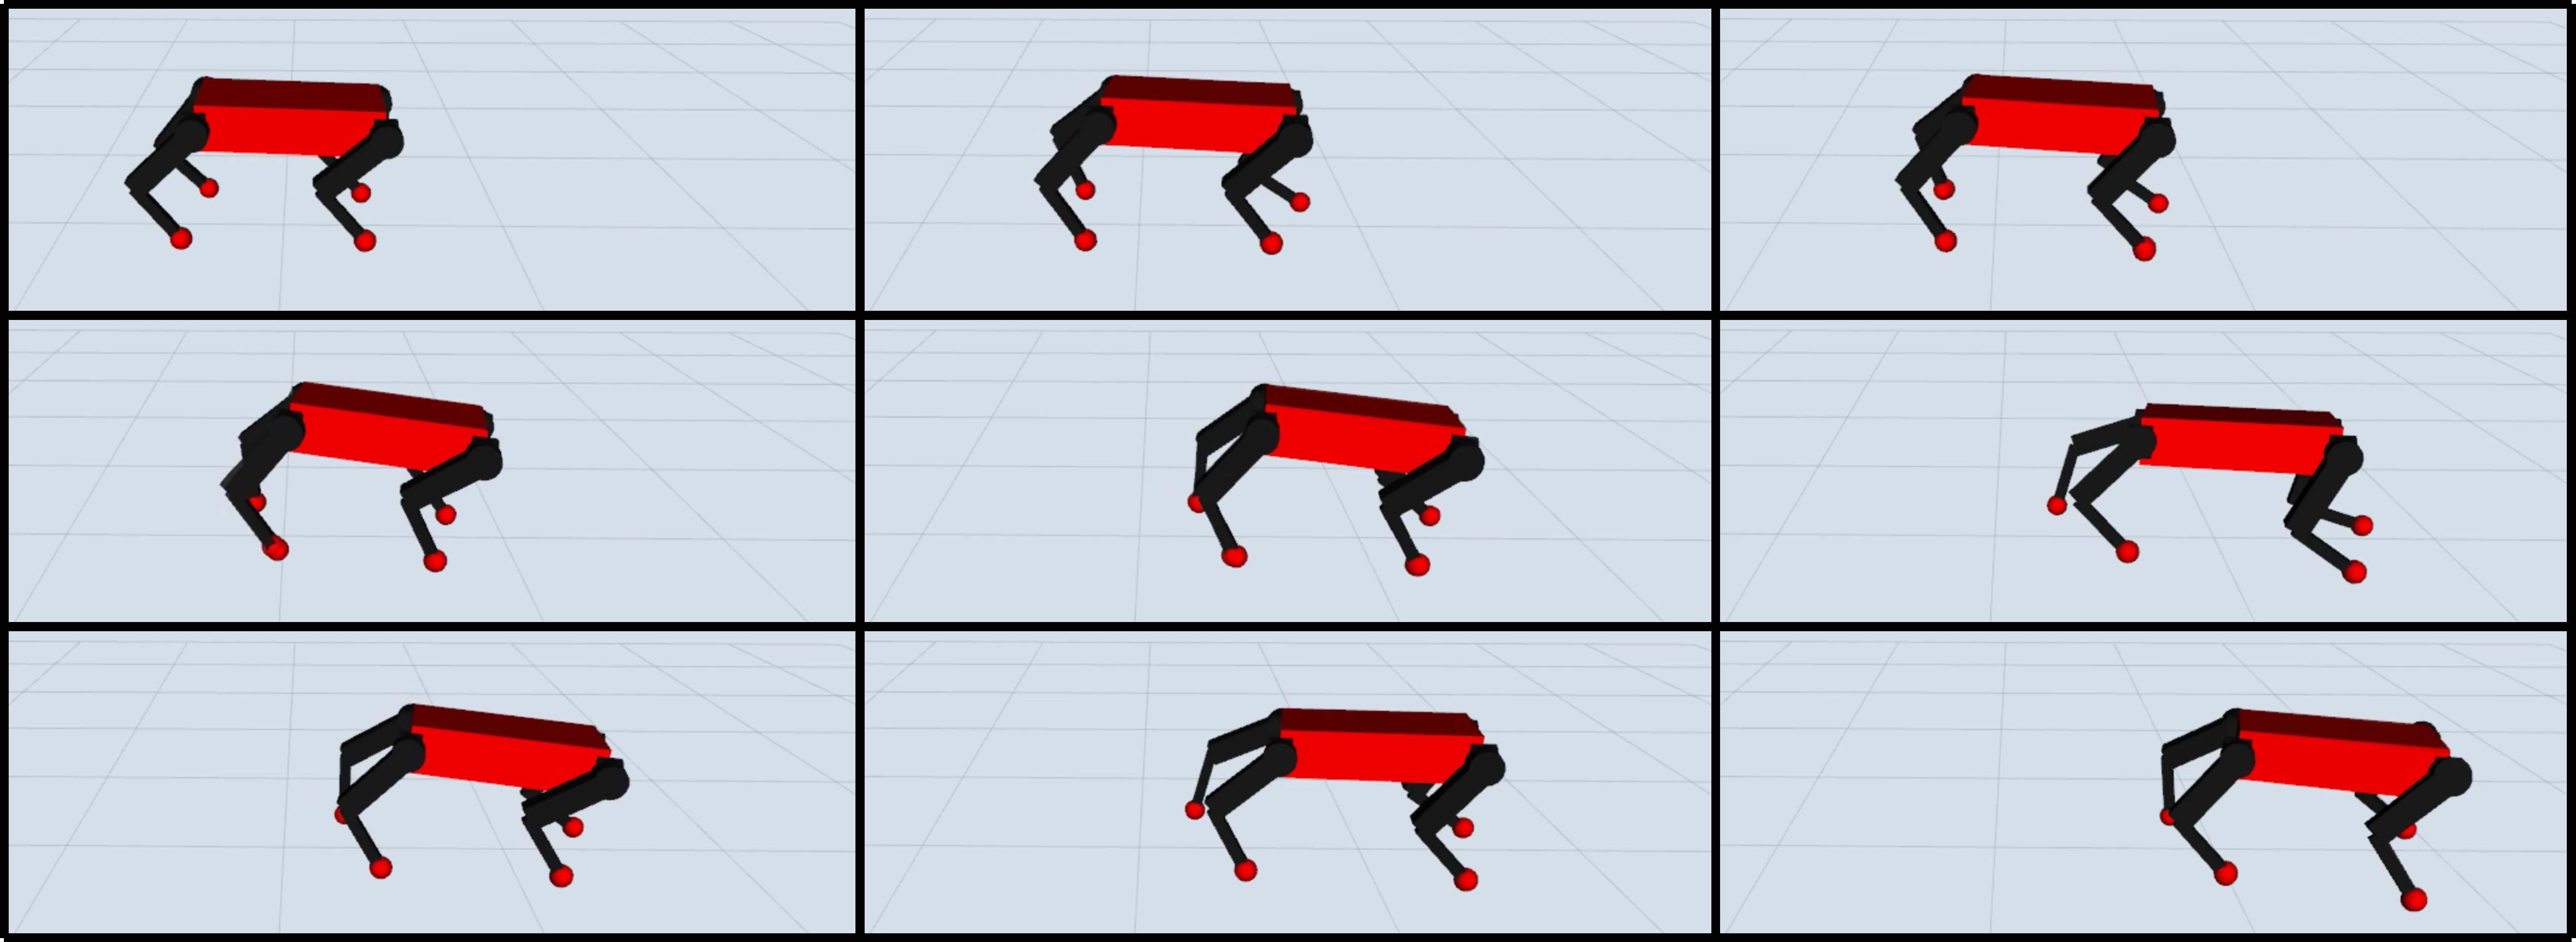
\includegraphics[width=0.9\columnwidth]{imgs/proof_of_concept.pdf}
	\caption{Preliminary results showing the agent learning to move the robot forward exploiting the underlying RHC controller, from right to left and from top to bottom.}
	\label{fig:proof}
\end{figure}
To showcase the potential of the proposed hybrid RL-RHC approach and of our framework, we trained a RL agent using PPO~\cite{rl:schulman2017proximal} to exploit a RHC controller for achieving a very simple forward locomotion task on a quadruped robot (shown in Fig.~\ref{fig:proof}). The agent is given a forward velocity reference to track and is continuously rewarded based on the task error and the performance of the underlying RHC controller. We observe the emergence of completely acyclic contact phases, varying from crawling to bound-like patterns.
 